\documentclass[11pt,a4paper,UTF8]{zhalabReport}


\title{\fontsize{40}{60}\selectfont 动态场景下的SLAM\\相关技术总结报告}
%\author{ 作者 Author }
\date{\chdate\today}

%!TEX program = xelatex

\newcommand{\setmode}[1]{\def\mode{#1}}
%\setmode{final} % final OR draft
\setmode{draft} % final OR draft
\long\def\IGNORE#1{} \long\def\COMMENT#1{}
\def\authornote#1#2#3{{\textcolor{#2}{\textsl{\small#1:[*#3*]}}}}
\ifthenelse{\equal{\mode}{draft}} {
	\newcommand{\zknote}[1]{\authornote{ZK}{red}{#1}} % Zike
	\newcommand{\wxnote}[1]{\authornote{WX}{green}{#1}} % Xin
	\newcommand{\rknote}[1]{\authornote{RK}{cyan}{#1}} % Qiao
	\newcommand{\pjnote}[1]{\authornote{PJ}{magenta}{#1}} % PJ
	\newcommand{\zsnote}[1]{\authornote{ZS}{yellow}{#1}} % Zsh
	\newcommand{\sknote}[1]{\authornote{SK}{blue}{#1}} % Shunkai
} {}

\ifthenelse{\equal{\mode}{final}} {
	\newcommand{\zknote}[1]{}
	\newcommand{\wxnote}[1]{}
	\newcommand{\rknote}[1]{}
	\newcommand{\pjnote}[1]{}
	\newcommand{\zsnote}[1]{}
	\newcommand{\sknote}[1]{}
	\typeout{************* MODE: Final}
} {}



\begin{document}
%%%%%%%%% ABSTRACT

\maketitle

\tableofcontents
%%%%%%%%% BODY


\chapter{动态环境下的SLAM系统}



\label{sec:slam}
\subsection{基于运动分割的SLAM技术}
\label{subsec:motion_segmentation}

动态分割(又称为移动物体检测/分割\cite{Derome2015Moving, Klappstein2008Moving, Kundu2009Moving})透过将特征区分为两类特征,静态和动态特征,以检测图像中移动的区块。
明确地说,给定在图像空间中的特征点集合,动态分割将特征点聚类为静态集合和动态集合。
传统的视觉SLAM使用鲁棒的静态方法,计算几何模型(如基本矩阵、单应矩阵)来实现动态分割。
比如利用随机抽样一致算法(RANSAC)\cite{Fischler1981Random}和特定的距离度量方法(如桑普森距离\cite{Hartley2008Multiple})将不服从模型的点剔除。
当静态的特征点占了主体时,这种方法能够有很好的效果。
当动态物体占了相机的绝大部份, 或是捕捉到的场景被巨大的移动物体遮挡时,这种方法可能就会失败。
其他方法结合其他传感器来解决这个问题,如使用惯性测量单元(IMU)估计相机自身的运动\cite{Jones2011Visual, Leutenegger2014Keyframe}。
通过IMU得到的位姿估计可以用来初始化相机位姿并且鲁棒地分割静态和动态特征。
在这一章节,我们讨论传统视觉SLAM和视觉惯性SLAM之外,分割静态和动态物体的其他方法。

\subsubsection{背景--前景初始化}
背景-前景初始化技术假设系统有对于环境的先验知识,利用这个信息分割静态和动态特征。这个先验知识可以归于背景( 静态特征)或是前景( 动态特征)。
如果系统的先验知识是关于前景目标,表示系统知道相机前方运动物体的类型或形状。

大部分前景初始化的实现方法使用tracking-by-detection结构\cite{Breitenstein2010Online, Lee2014Driving}。Wangsiripitak等人\cite{Wangsiripitak2009Avoiding}假设对于一个三维物体,它的动态特征的位置是已知的。他们用边上的控制点集建模一个三维多面体模型,然后使用Harris’s RaPid tracker\cite{Harris1990RAPID}对其进行跟踪。如果之前跟踪的特征位于跟踪中的三维多面体上,当检测到这个物体处于移动状态时,便将特征剔除。被这个物体遮挡的静态特征也会被剔除。相似地,Wang等人\cite{Wang2010Visual}假设移动中的物体上的SURF特征描述子\cite{Bay2008Speeded}是已知的并存在数据库中。通过比较在特征检测步骤得到的描述子,就可以识别移动中的物体,也可以估算它的位移和旋转。Chhaya等人\cite{Chhaya2016Monocular}使用deformable wireframe object class model对建模相机前方的车辆。这个模型使用Principal Component Analysis (PCA) 在3D CAD data上训练而得。这个模型用在位姿估计得过程将车子识别并分割出来。另一方面,Lee等人\cite{Lee2014Driving, Lee2016Ground}基于tracking-by-detection结构,他们使用Constrained Multiple-Kernel(CMK)法,利用深度信息处理跟踪过程中的遮挡问题,同时使用预训练的人类检测器来跟踪行人。

有别于初始化前景的物体,背景初始化类似于background subtraction技术,设定一个背景模型\cite{Babaee2017A,Piccardi2005Background}。Zhang等人\cite{Zhang2012Visual}初始化属于背景的特征点集合,并令这个集合为背景的模型。他们假设当首次进行视觉的初始化时,是没有前景物体的。当经过新的一帧后,使用GPCA\cite{Ren2005Generalized}进行三维动态分割。分割出来的动态部分,对于先前的背景模型具有最高响应值部分,将会用来更新背景。根据新的背景模型,运用标准的对极几何法估计位姿。

\subsubsection{几何约束}
由于动态的特征会违反静态场景中的多视角几何约束,依赖此约束的技术是利用极限几何的性质\cite{Hartley2008Multiple}来分割静态和动态特征。这些约束可以从极线、三角化、基本矩阵估计或重投影误差的等式中得出。

Kundu等人\cite{Kundu2009Moving}根据机器人里程计构建一个基本矩阵来定义两个几何约束。第一个约束是极线几何约束,在随后的视角下,成功匹配的点应该要在对应的极线上。如果跟踪到的特征离极线过远,就会被认为是动态特征。第二个约束是Flow Vector Bound(FVB),目的是分割当三维点沿着极线移动时产生的退化运动。通过设定跟踪到的特征流的上界和下界,超过这个范围的特征就会被作为运动的特征检测出来。最后通过循环的贝叶斯滤波器决定将特征分类为静态特征或动态特征。不同于使用极线约束,Migliore等人\cite{Migliore2009Use}利用三角化的原理分割静态和动态特征。他们在概率滤波器的框架下,持续地检查三个不同视角投影出来的视线的交点。如果特征是动态的,则这个交点在运动的过程中不会一样,甚至不会产生交点。但是由于传感器存在的噪声,他们使用Uncertain Projective Geometry\cite{Heuel2001Matching},将测量的不确定性加入他们检查不同视线关系的过程。最后通过统计假设测试\pjnote{statistical hypothesis test}分类静态和动态的特征。

将移动的物体误分类为静态物体并将其加入位姿估计,将会严重地使SLAM系统的性能降低,Lin等人\cite{Wang2007Simultaneous}通过观察这一性质来检测移动中的物体。他们计算两种不同条件下的位姿估计之间的差异,其中一个不加入新检测到的特征,另外一个假设新检测到的特征是静态的并加入位姿估计。借由计算两个结果的距离,设定一个门槛,通过二分贝叶斯滤波器整合,就能够精确地分割静态和动态的特征。

另外一个几何的方法是利用重投影误差。Zou和Tan\cite{Danping2013CoSLAM}将先前帧的特征投影到当前帧上,测量这些跟踪到到特征的距离。通过这个重投影的距离分类静态和动态的特征。Tan等人\cite{Wei2013Robust}使用同样的投影原理检测动态特征。他们同时将遮挡问题作为考量提出了一个鲁棒的视觉SLAM。在一个特征投影到当前帧上时,他们检测图像上的外观差异,也就是图像中的某一部分是否改变了。如果外观差异巨大,有极大的可能这个区域被动态物体遮挡,或是因为视点改变被静态物体所遮挡。因为上述原因被遮挡的三维点,会被保留并用来估算相机位姿。

\subsubsection{光流}
光流的定义了两个连续的图像间,图案亮度的表面运动\cite{Horn1980Determining}。通常它对应了图像的运动场,因此可以用于分割移动的物体。Klappstein\cite{Klappstein2008Moving}根据光流定义了运动度量描述移动中的物体的似然。测量当场景中有运动物体时,光流错误的范围。Graph-cut算法根据运动度量分割移动的物体。

Alcantarilla等人\cite{Alcantarilla2012On}通过运动似然残差得到的场景流(三维的光流)中的三维运动向量系数,分割移动物体。马氏距离用于考量基于稠密光流和双目重建计算场景流的测量不确定性。如果残差小,特征点很可能属于静态物体。在运动似然残差设立门槛,属于运动物体的特征点可以从SLAM过程中删除,使得视觉里程计的估计更鲁棒。Derome等人\cite{Derome2015Moving, Derome2014Real}计算预测的预想与双目相机观测得到的图像的残差,以此计算光流。预测的图像是根据估计的相机自身运动,将当前帧的双目图像转换到过去的帧上。接着从残差场上的斑点检测移动中的物体。

\subsubsection{相机运动约束}
一般的SfM和视觉SLAM通过8点的均值\cite{Longuet1981A}或5点法\cite{David2004An}计算相机的运动。这种普通的相机运动估计并没有考虑任何相机移动方式的假设。另外一种方式是假设相机根据特定参数提供的外在信息(如车轮里程计的信息)估计相机位姿。加入这种相机运动约束,通过匹配特征点是否符合相机运动的约束,分类静态特征。

Scaramuzza\cite{Scaramuzza20111}提出利用轮式车辆的非完整性约束计算相机运动的方法。他假设相机运动是平面或圆形的,以此建模相机运动。由此约束,相机运动可以被参数化为1自由度并且可由1点法计算\cite{Scaramuzza2009Real}。同样地,Sabzevari等人\cite{Sabzevari2016Multi}也利用阿克曼转向几何提供的轮式车辆约束来计算相机运动。满足估计的相机运动的特征点会被认为是静态特征,其他的特征点则被认为是动态特征。

\subsubsection{运动分割的深度学习}
在基于特征的运动分割中,我们知道可以利用光流分割移动中的物体。Dosovitskiy等人\cite{Fischer2015FlowNet}展示了光流的估计是可以通过有监督学习获得的。他们提出了两个不同结构的卷积神经网络(CNN)来预测光流。其中一个网络(FlowNetS)将两个连续帧的图像作为输入,而另一个网络(FlowNetC)将两个不同的CNN合并来比较两个特征地图。Ilg等人\cite{Ilg2017FlowNet}进一步提出了FlowNet 2.0,将FlowNetS和FlowNetC放入一个更深的网络,同时加入并行的网络来处理小的位移。实验表明FlowNet 2.0的结果可以与最新的方法并肩。Mayer等人\cite{Mayer2016A}延伸出了用双目图像计算场景流的方法。这个光流可以被放大更深的网络,检测运动特征\cite{Gladh2016Deep}。这些运动特征对于动作识别非常有用\cite{Gkioxari2014Finding,Simonyan2014Two}

Lin和Wang\cite{Lin2014Deep}构建了一个可以显式地在图像空间分割移动物体的网络,他们使用Reconstruction Independent Component Analysis(RICA)自编码器\cite{NIPS2011_4467,Le2013Building}来学习时空特征,但是由于时空特征无法学习运动的三维几何信息,因此仍然使用几何特征帮助分割任务。几何特征和时空特征都放进循环神经网络(RNNs)来计算最终的运动分割。Fragkiadaki等人\cite{Fragkiadaki2015Learning}将RGB图像和光流的置信度\pjnote{objectness score??}。类似于AlexNet\cite{Krizhevsky2012ImageNet}的两个并行网络用来处理RGB图像和光流,接着放入回归网络生成运动估计\pjnote{motion proposal}。Valipour等人\cite{Valipour2017Recurrent}提出了Recurrent Fully Convolutioal Network(R-FCN),使用时序数据在线地在图像序列分割前景物体。Fully Convolutional Network(FCN)\cite{2014arXiv1411}用于学习空间特征和生成像素的稠密预测,但是Gated Recurrent Unit(GRU)用于在反卷积之前对时间特征进行建模。
© 2019 GitHub, Inc.

\section{基于运动物体跟踪的SLAM技术}
\label{subsec:object_tracking}

动态物体分割和3D跟踪会基于运动将特征对应关系分成不同的组,并且三维地跟踪它们的轨迹。基于特征的用于动态对象分割的技术的输入仅由完整特征或动态特征组成。另一方面,基于深度学习的方法可以直接处理图像序列,然后分割后的动态对象会被送到3D跟踪模块中以获得对象轨迹,也可以可选地利用相机自我运动或从动态对象3D跟踪模块获得的3D点云来帮助跟踪过程。3D点云的可用性可以使输出对象轨迹与静态世界一致。本节讨论分割和跟踪动态对象的技术。

\subsection{动态物体分割}
动态对象分割(也称为多体运动分割或eorumotion分割)将所有特征对应分成$n$个不同的对象运动聚类。由于这个问题类似于鸡生蛋蛋生鸡问题,所以它被认为是一个难题。为了估计对象的运动,应首先对特征进行聚类;另一方面,聚类特征需要所有移动物体的运动模型。由于遮挡,运动模糊或丢失跟踪特征,噪声、异常值或缺少特征对应性使问题更加复杂。另一个挑战是处理退化运动(如当物体与相机在相同平面上以相同方向和速度移动时)或相关运动(例如两个人一起移动,关节运动)。本节讨论处理此问题的现有方法。

\paragraph{静态模型分割}
在静态场景中,可以通过一个运动模型来描述连续图像之间的特征点的变换。相比之下,动态场景中的特征点可能来自多个运动模型,每个运动模型与不同的物体相关联。运动模型可以基于以下模型之一:基本矩阵($F$),仿射基本矩阵($F_A$),本质矩阵($E$),单应性/投射性($H$)或仿射性($A$)。选择模型时会尝试将所有可能的运动模型与数据拟合,并选择最适合数据的模型。如果数据可以由动态场景中的几个模型描述,则基于这些运动模型,需要很多假设进行分割数据。\\

基于统计技术的3D运动分割方法会对数据的子集进行采样,并将运动模型拟合到RANSAC~\cite{fischler1981random}
或Monte-Carlo采样迭代~\cite{schindler2006two}
下的采样数据集中。运动模型用于构建内部集合,并将剩余数据排除为模型的异常值。然后,再次对剩余数据(先前模型的异常值)进行采样,以找到并拟合能够最佳描述剩余数据的另一模型。重复该过程,直到所有数据都可以由$n$个运动模型描述,或者剩余的异常值不足以产生更多的运动模型。可以从头开始重复该运动分割过程以生成许多候选假设。\\

基于信息标准,我们可以确定哪种模型最适合描述数据。文献中存在若干信息标准。Akaike的信息准则(AIC)~\cite{akaike1998information}
选择能够将似然函数最大化,但将用以生成模型的估计参数的数量最小化的模型。由于最大似然估计总是选择最通用模型作为最佳拟合模型,对于参数数量的惩罚正是基于这一点~\cite{faugeras1998geometric}
。一个直观的例子是,相对于某点的任何点的误差都高于或等于相对于线的误差; 因此,一条线始终会是作为描述数据点的最佳模型。AIC通过平衡拟合优度与模型复杂性来解决这个缺点。它具有以下形式:
\begin{equation}
AIC=(-2)log(L)+2K,
\end{equation}
其中$L$是对数似然函数,$K$是模型的参数个数。通常通过估计似然函数,将基于特定距离度量(例如重投影误差或Sampson距离近似)观察对应关系的可能性最大化~\cite{hartley2000multiple}
。然后,AIC选择在最小AIC估计(MAICE)过程下具有最小AIC分数的模型。\\

尽管AIC很受欢迎,但它没有渐近一致的估计值,并且容易过度拟合,因为它没有考虑到观测的数量。Schwarz~\cite{schwarz1978estimating}
提出了一种使用贝叶斯定理的修正,称为贝叶斯信息准则(BIC)。
BIC通过基于先验的复杂性对先验进行建模来扩展观察数据的后验概率。另一方面,Rissanen~\cite{rissanen1984universal}
提出最小描述长度(MDL),通过使用最小位表示来最小化数据的编码长度。基于先前工作的局限性,Kanatani~\cite{kanatani2005statistical}~\cite{kanatani2001motion}
通过考虑观察的数量和模型的维度,提出了几何信息准则(G-AIC,或在一些文献中称为GIC);它有以下形式:
\begin{equation}
GIC=(-2)log(L)+2(DN+K),
\end{equation}
其中$N$是数据的数量,$D$是模型的维数(例如,单应性有二维,基本矩阵有三维)。基于BIC的另一个扩展是由Torr~\cite{faugeras1998geometric}
设计的几何鲁棒信息准则(GRIC),结合了处理异常值的鲁棒性和处理不同维度的能力。GRIC具有以下形式:
\begin{equation}\label{GRIC}
GRIC=(-2)log(L)+DNlog(R)+Klog(RN),
\end{equation}
其中$R$是数据的维度。\\

有不同的方法来实现3D运动分割的统计模型选择。Torr~\cite{faugeras1998geometric}
对邻近的特征对应进行采样,并在RANSAC迭代下计算不同的运动模型(F,FA,H,A)。GRIC用于选择适合特定内部聚类的最佳运动模型。然而,当所选模型的内部数量低于阈值时,则会应用期望最大化(EM)。为了避免昂贵的暴力采样计算,Schindler和Suter~\cite{schindler2005two}~\cite{schindler2006two}
提出局部蒙特卡罗采样,从图像上定义的子区域中提取样本。他们提出了一种从数据中估计噪声标度的方法,从而可以恢复每个运动的残差分布及其标准差。此外,他们导出了一个新的似然函数,允许运动模型(F,H)重叠,而由GRIC选择最佳模型,如公式\ref{GRIC}所示。\\

虽然之前的方法是对两个图像序列进行操作,但Schindler等人~\cite{schindler2006perspective}
将~\cite{schindler2005two}
中的技术扩展到一般运动模型(基本矩阵$E$)下的几个透视图像。为了从多于两张图像的序列中关联若干本质矩阵备选,他们通过仅连接那些具有相似内点集的基本矩阵,来加强时间一致性。最后,使用类似MDL的方法来选择描述运动的最佳模型。这种方法已被广泛用于Schindler等人的任何相机模型(不仅是透视相机)和运动模型(不仅是基本矩阵E)~\cite{schindler2008model}。
Ozden等人也考虑了实际因素~\cite{ozden2010multibody},
他们处理了如何将先前移动的对象与背景合并,或如何将聚类分成两个不同的运动的问题。\\

Thakoor等人~\cite{thakoor2010multibody}
将模型选择问题描述为组合优化问题。采用分支限界技术,通过将优化问题分解为较小的子问题,使用AIC作为代价函数来优化运动分割。对应的局部采样也用于产生运动,而空假设用于处理异常值。最近,Sabzevari和Scaramuzza~\cite{sabzevari2014monocular}
通过投影轨迹矩阵框架的分解运用了统计模型选择技术。极线几何用于生成运动模型,而重投影误差用于拒绝无效假设。假设通过迭代地细化结构估计和运动分割来被评估。这已经在~\cite{sabzevari2016multi}
中通过强制执行自运动约束被扩展,使得可以通过分别使用单点算法~\cite{scaramuzza20111}~\cite{scaramuzza2009real}
和两点算法~\cite{ortin2001indoor}
来计算相机运动和运动物体运动。\\


\paragraph{子空间聚类}
子空间聚类是基于以下观察而被提出的:许多高维数据可以由低维子空间的并集来表示。数据点的子空间可以表示成基础向量和数据的低维表示。子空间聚类框架下的三维运动分割问题基本上是找到与每个物体运动相关的每个子空间,并将数据拟合到子空间中。然而,由于子空间和数据分割在实际中是未知的,因此估计子空间参数并将数据聚类到不同的子空间应该同时进行。最初Costeira-Kanade~\cite{costeira1998multibody}
和Gear~\cite{gear1998multibody}
指出,这个问题是基于独立的刚体运动位于线性子空间中这一观察的。通过强制执行排名约束,可以恢复每个线性子空间。\\

Kanatani~\cite{kanatani2001motion}
提出“子空间分离”作为聚类低维子空间的一般方法(不仅限于运动分割),借用统计模型选择的原理来完成子空间分离,但是运用在子空间而不是运动模型上。AIC通过平衡在拟合数据点到子空间时残差的增加,与在将两个子空间合并为一个组时自由度的减小,来选择最佳子空间配置,并使用最小平方的中值(least median of squares)来拟合包含异常值的数据点。不同的是,Vidal等人~\cite{vidal2005generalized}
提出广义主成分分析(GPCA)作为PCA的扩展。虽然PCA仅用于位于线性子空间中的数据,但GPCA将问题推广为由多个线性子空间产生的数据点。GPCA通过多项式嵌入(或Veronese映射)将$n$次齐次多项式拟合到数据中,并通过计算特定点处多项式的导数来找到每个子空间的法线,以解决寻找子空间的问题。然后,通过从法向量之间的角度计算相似性矩阵,并使用谱聚类对其进行聚类来获得分割。为了在运动分割中考虑实际情况,在执行聚类之前,他们通过将数据投影到较低维空间中来扩展~\cite{vidal2005generalized}
。然后,可以通过找到多项式嵌入的秩来计算运动的数量$n$。\\

由于之前的工作假设运动是刚性的,Yan和Pollefeys~\cite{yan2006general}
提出了一个称为局部子空间亲和力(LSA)的通用框架,可以用于独立,铰接,刚性,非刚性,退化以及非退化运动。LSA通过对点及其最近邻近点进行采样并将局部子空间拟合到采样数据来估计子空间,其中可以通过计算矢量之间的角度或距离找到最近的邻近点。然后,亲和矩阵作为衡量两个局部子空间的主要方面被计算,并且谱聚类应用于亲和矩阵后聚类完成。在估计子空间之前,还要进行向较低维子空间的投影。与LSA类似,Goh和Vidal~\cite{goh2007segmenting}
也将局部子空间拟合到一个点及其最近邻近点。该方法称为局部线性流形聚类(LLMC),是基于局部线性嵌入(LLE)~\cite{saul2003think}
算法开发的。他们通过使用LLE将数据转换为低维表示,并计算由LLE产生的矩阵的零空间来将与每个运动相关联的分离的流形进行聚类,而其中数据的分离可由零空间中的向量表示。\\

Elhamifar和Vidal~\cite{elhamifar2009sparse}~\cite{elhamifar2013sparse}
给出了另一种观点,它利用稀疏的表示来将运动进行聚类。他们发现线性或仿射子空间的并集中的点可以表示为子空间中所有数据点的线性或仿射组合,提出了稀疏子空间聚类(SSC)。然而,只有当该点可被表示为位于同一子空间中的数据的线性或仿射组合时,才能获得最稀疏表示。在无噪声数据下,可以通过求解$L_1$最小化问题来估计最稀疏系数。给定最稀疏系数,可以构建亲和度矩阵,并且可以通过谱聚类来完成聚类。Rao等人开发了SSC的扩展~\cite{rao2009motion}
。它们融合了稀疏表示和数据压缩以处理实际问题,例如数据丢失,不完整或包含异常值。最近,杨等人~\cite{yang2015sparse}
还通过为缺少条目的数据提出各种矩阵补全技术来改进SSC。刘等人~\cite{liu2012robust}
和陈等人~\cite{liu2010robust}
没有使用稀疏表示而是采用低秩表示(LRR),使用谱聚类来定义用于子空间分割的亲和矩阵。\\

值得注意的是,大多数子空间聚类技术以批处理模式运行。Vidal~\cite{vidal2007online}
设计了一种迭代聚类技术,用于位于多个移动超平面中的数据。他用一组时变多项式模拟了一组移动超平面,通过估计标准化梯度下降框架内的超平面的法向矢量来递归地完成分割。Zhang等人提出了在线子空间聚类的另一种实现方式~\cite{zhang2009median}
。他们修改了K-flats算法,使其能够逐步获取输入数据。他们将$L_1$用作目标函数而非$L_2$,以便在噪声和包含异常值的数据下提高其性能。\\

在过去的几十年中,子空间聚类已经成为一个被广泛研究的主题,并且不同的研究团体已经开发了许多方法。有几个与子空间聚类相关的调查论文,涵盖了从一般技术到关注运动分割和面部聚类的应用。有关子空间聚类的更详细回顾,感兴趣的读者可以关注~\cite{vidal2011subspace}。\\

\paragraph{几何法}
几何法将多个视图的几何的标准公式从静态场景扩展到包含独立移动对象的动态场景中。虽然有一个基本矩阵描述了摄像机相对于静态场景的一般运动,但在动态环境中,将有$n$个基本矩阵描述$n$个物体的运动,其中包括一个用于静态特征的运动。Vidal等人~\cite{vidal2006two}通过提出多体极线约束来宏观地研究这个问题。给定$x_1$和$x_2$分别作为第一和第二图像之间的特征对应关系,$x_2^TFx_1=0$表示静态场景的极线约束,其中$F\in{\mathbb{R}^{3\times3}}$是基本矩阵。如果场景包含$n$个独立的移动对象,则存在与每个移动对象相关联的一组基本矩阵$\{F_i\}_{i=1}^n$,使得满足以下多体对极约束~\cite{vidal2002segmentation}:
\begin{equation}\label{con:epsilon}
\varepsilon(x_1,x_2)\doteq\prod_{i=1}^n(x_2^TF_ix_1)=0.
\end{equation}
该多体极线约束将标准极线约束方程从双线性变换为n阶的齐次多项式(在$x_1$和$x_2$中)。通过使用veronese映射$v_n:\mathbb{R}^3\to\mathbb{R}^{M_n}$将多项式方程映射到包含$M_n$单项式的向量中,可以将该齐次多项式方程再次转换为双线性问题,其中$M_n\doteq\binom{n+2}{n}$。 因此,可以将等式\(\ref{con:epsilon}\)中的多体极线约束转换成
\begin{equation}\label{vn}
v_n(x_2)^T\tilde{F}v_n(x_1)=0,
\end{equation}

其中$\tilde{F}$是多体基本矩阵,是所有基本矩阵的对称张量积表示~\cite{vidal2006two,vidal2002segmentation}。如果$n$是已知的,通过使用Kronecker乘积重新排序$v_n(x_1)$和$v_n(x_2)$的条目并将$\tilde{F}$的行堆叠到$f\in{\mathbb{R}^{M_n^2}}$,可以将等式\(\ref{vn}\)转换为$f$中的线性方程,并且可以是通过最小二乘估计进行估计。然后通过多体核线$\tilde{l}\doteq\tilde{F}v_n(x_1)\in{\mathbb{R}^{M_n}}$的多项式因子分解找到与每个运动相关的核线,可以恢复各个基本矩阵$F_i$。随后,动态特征的运动分割可以通过将每个特征对应与正确的基本矩阵对齐来完成~\cite{vidal2002segmentation}。\\

Vidal和Hartley~\cite{vidal2007three}通过引入多体三线性约束和多体三焦张量,将多体SfM公式从两个视图扩展为三个视图。它是从静态场景到包含多个对象的动态场景的三线性约束和三焦张量~\cite{hartley2000multiple,torr1997robust}的推广。通过嵌入如等式\(\ref{vn}\)中的特征对应关系并使用最小二乘法估计,可以线性地求解多体三焦张量。通过计算其二阶导数,从多体三线性约束中恢复对应于每个对象的每个三焦张量。\\

\paragraph{用于动态对象分割的深度学习方法}
用于解决动态对象分割问题的DNN的当前工作依赖于预定义数量的刚体运动。可以从3D点云数据或光流导出用于产生密集对象掩模(dense object masks)的网络及其相关的成本函数。Byravan和Fox~\cite{byravan2017se3}
引入“SE3-Net”作为DNN,能够分割预定义的,以来自3D点云的$SE(3)$变换表示的$n$个动态对象。其中构造了卷积/反卷积编码器-解码器网络来预测对象掩模和每个对象的刚体变换。编码器由两个并行卷积和全连接的网络组成,它们分别从点云产生潜在变量并对控制矢量进行编码。解码器通过两个并行去卷积和全连接网络处理来自编码器的级联输出,产生逐点对象掩模,并且处理$SE(3)$变换。变换层用于融合3D点云数据,对象掩模及其$SE(3)$以生成用于数据训练的预测点云。\\

Vijayanarasimhan等~\cite{vijayanarasimhan2017sfm}
利用光流来使用DNN分割动态对象。他们设计了一个名为“SfM-Net”的网络,这是一个几何感知网络,能够预测深度,摄像机运动和动态对象分割。这些网络由两个流卷积/反卷积子网组成,充当结构和运动网络。结构网络学习预测深度,而运动网络估计相机和物体运动。虽然物体运动是由CNN产生的嵌入层顶部的两个全连接层计算而来,但是动态对象分割是通过将嵌入层送到去卷积网络来预测的。然后,根据相机和物体运动从深度预测变换点云,然后将变换的点云重新投影到图像空间中,将来自结构和运动网络的输出转换成光流。通过使用这种技术,可以通过最小化光度误差来实现自监督网络。\\



\subsection{动态物体的3D跟踪}
已知3D坐标中移动物体的位置(包括深度信息),在3D中跟踪动态物体的问题是很重要的。挑战在于视觉SLAM中用于估计场景的3D结构的标准方法,即三角测量~\cite{hartley1997triangulation}
,对于动态对象不起作用,因为从相应的特征点反投影的光线不相交。给定$x_1$和$x_2$分别作为来自第一帧和第二张帧图像的特征对应关系,应该能够通过经由它们的相关联的相机投影矩阵$P_1$和$P_2$交叉$x_1$和$x_2$的背投影光线来计算相应的3D点$X$。由于物体是独立运动的(来自相机运动),因此从第一帧到第二帧的投射光线也在移动,因此不相交,需要替代技术来解决这个问题。本节讨论恢复在摄像机前移动的物体的3D轨迹的现有方法。

\paragraph{轨迹三角测量}
标准三角测量~\cite{hartley1997triangulation}
不能用于重建运动物体的3D结构,因为反投影光线不相交。Avidan和Shashua~\cite{avidan1999trajectory}~\cite{avidan2000trajectory}
提出了轨迹三角测量的方法,作为在物体轨迹已知或满足参数形式时重建运动物体的3D点的技术。他们假设3D点沿着未知的3D线移动,然后重建问题变成找到与来自$t$个视图的投射光线相交的3D线的问题。为了获得唯一的解决方案,至少需要$t=5$,因为来自三个视图的交叉线组将形成二次曲面,使得来自第四视图的光线在两个点处相交。因此,五个视图产生了唯一的解决方案。\\

$$此处跳过一段公式及文字$$

Shashua等人~\cite{shashua1999trajectory}
假设物体在圆锥截面上移动,而没有假设物体沿着一条线移动。这时需要9个视图才能获得唯一的解决方案,尽管如果已知圆锥曲线的类型有七个视图就足够了,例如3D欧几里德空间中的圆。他们通过将随机圆锥拟合到2D空间中的运动点或通过最小化3D中估计的圆锥半径的误差来解决非线性优化问题,从而可以实施先验约束。基于以前的工作,Kaminski和Teicher~\cite{kaminski2002general}~\cite{kaminski2004general}
通过将曲线表示为投影空间中的超曲面族来推广轨迹三角测量。这种多项式的表示将非线性轨迹问题转换为未知参数中的线性问题。另一方面,为了处理缺失的数据,Park等人~\cite{park20103d}
将3D轨迹表示为轨迹基矢量的线性组合,这样就可以使用最小二乘法鲁棒地估计3D点的恢复。他们还通过分析自我运动,点运动和轨迹基矢量之间的关系提出了可重构性标准。由于可重构性与3D重建误差成反比,因此该标准可以准确地考察精确重建的可能性~\cite{park20153d}。\\

\paragraph{粒子滤波器}
由于可观测性问题(观察者与目标之间的距离无法被观测),使用单目相机在3D中跟踪运动物体的问题可被视为仅承载跟踪(BOT)问题。单目摄像机可以被视为BOT传感器,因为它只能提供被移动物体上的被跟踪特征点的方向信息(例如,前一帧中的观察特征与相对于摄像机中心的当前帧之间的角度)。基于滤波器的方法对于BOT问题是优选的,因为它可以模拟观察者和目标的位置和速度的不确定性,并且已被作为目标运动分析问题广泛研究~\cite{aidala1983utilization}~\cite{le1998bearings}。\\

Kundu等人~\cite{kundu2011realtime}
采用粒子滤波器来估计移动物体的位置和速度。其中瞬时匀速运动模型和李代数分别用于模拟未知运动和参数化对象的刚性变换。在初始化中,移动对象通过几何约束和流向量绑定(FVB)进行分割,如~\cite{kundu2009moving}
和~\cite{kundu2010realtime}
所示,并且粒子沿投影光线均匀分布。利用由静态场景3D点云估计得到的地平面和允许的最大深度值来约束粒子的空间。对于重要性采样,通过将每个粒子投影到当前帧中并计算与实际特征位置相比的投影误差来更新粒子的权重。由于具有较低误差或较高权重的粒子具有较高的重采样概率,因此它们集中于能够产生最小重投影误差的深度值周围。


\subsection{基于运动物体跟踪的SLAM技术}
\label{subsec:object_tracking}

\subsubsection{深度学习方法用于动态物体分割}
随着深度学习在越来越多的计算机视觉任务中表现出优异的性能,近年来也有不少研究将深度学习用于解决动态物体的分割问题。

在动态物体分割的研究中,许多学者使用了空间变换网络(Spatial Transformer Networks)~\cite{2015spatial}。这是因为动态物体分割的过程中涉及动态物体的识别,而同一类物体的大小、位置、姿态往往在不同图片中不尽相同,因此需要网络能抵抗这些因素的干扰,准确识别出物体,即网络的识别需要有空间不变性(spatially invariant)。而空间变换网络能以自监督学习的方式在网络内部对空间数据进行变换处理,使其具有空间不变性。该网络结构可作为一个模块嵌入到任何物体识别、检测、分割网络中,提高网络的性能。

由于动态物体分割本质上是将视频流中的动态物体识别、分离的过程,因此它可用深度学习中的注意力机制(attention)解决。近年来,出现了许多将注意力机制用于动态物体分割的研究工作,例如~\cite{2014multiple}用强化学习的方式训练循环神经网络(recurrent neural network, RNN),引入注意力机制使其输出图片中的多个物体。

目前,深度学习用于动态物体分割的研究工作往往需要预定义刚体的类型、运动模式或数量。将三维点云或光流作为输入,深度网络预测出动态物体的掩膜。Byranvan和Fox等人提出了SE3-Net~\cite{se3},能够从三维点云中将预先定义好的$n$个动态物体的6自由度位姿以$SE(3)$的形式预测出来。SE3-Net设计了一个编码-解码网络,使用卷积和反卷积预测每个动态物体的掩膜和6自由度位姿。其中,编码网络由两个并行的卷积和全连接网络构成,将输入的三维点云分别变换成隐变量和控制向量(control vector)。随后,将隐变量和控制向量拼接起来,由解码器(同样由两个并行的反卷积和全连接网络构成)输出稠密的物体掩膜和$SE(3)$变换参数。最后,用一个非线性变换层将三维点云、物体掩膜和$SE(3)$变换融合,生成动态物体的三维点云。

\begin{figure}[htbp]
	\centering
	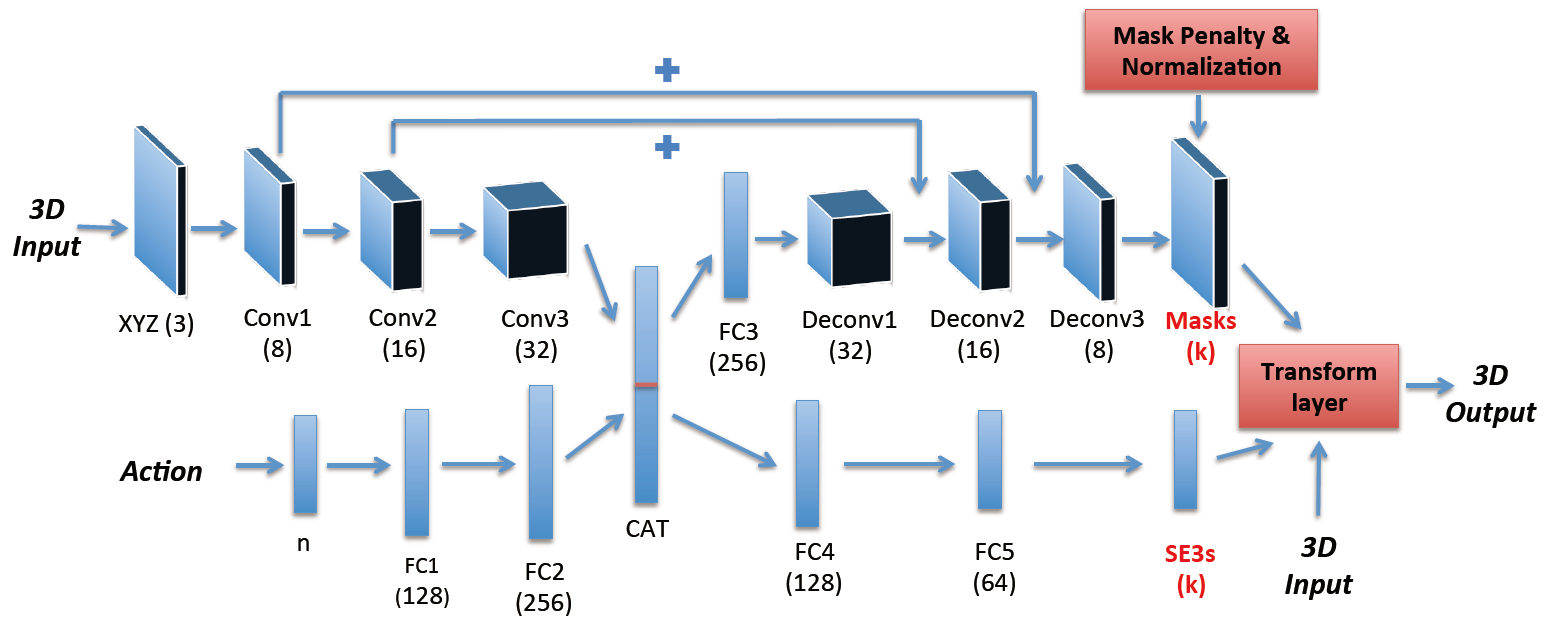
\includegraphics[width=0.9\textwidth]{figs/1-2/se3-net.png} 
	\label{se3-net}
	\caption{SE3-Net的网络结构图}
\end{figure}

Vijayanarasimhan等人通过实验证明,可以借助光流用深度学习分割场景中的动态物体~\cite{2017sfm}。他们设计了SfM-Net,通过显式的几何约束训练网络,使其可预测场景深度、相机运动和动态物体分割。SfM-Net由两个主流的卷积、反卷积网络构成,它们分别作为结构网络(structure network)和运动网络(motion network)。其中,结构网络通过学习预测场景深度,运动网络估计相机和物体位姿。在经过卷积网络的嵌入层(embedding layer)之后,通过两个全连接层输出动态物体的位姿估计。同时,嵌入层经过反卷积输出运动物体的掩膜估计。之后,通过估计的深度图,利用估计的相机和物体位姿将一帧RGB图像中的像素变换到另一帧的视角下,合成新视角下的图片,从而计算场景的光流。利用显示的几何约束关系,便可以自监督学习的方式通过最小化光度误差(photometric error)进行训练。

\begin{figure}[htbp]
	\centering
	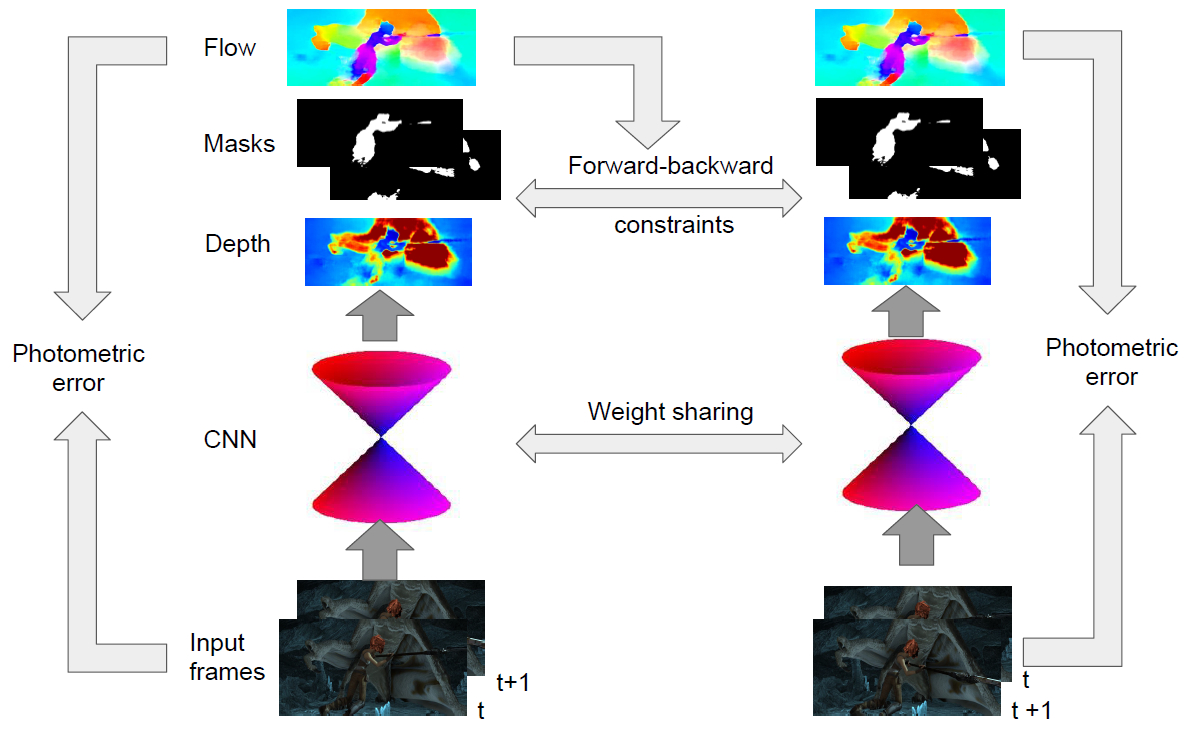
\includegraphics[width=0.7\textwidth]{figs/1-2/sfm-net.png} 
	\label{sfm-net}
	\caption{SfM-Net的流程图}
\end{figure}

\begin{figure}[htbp]
	\centering
	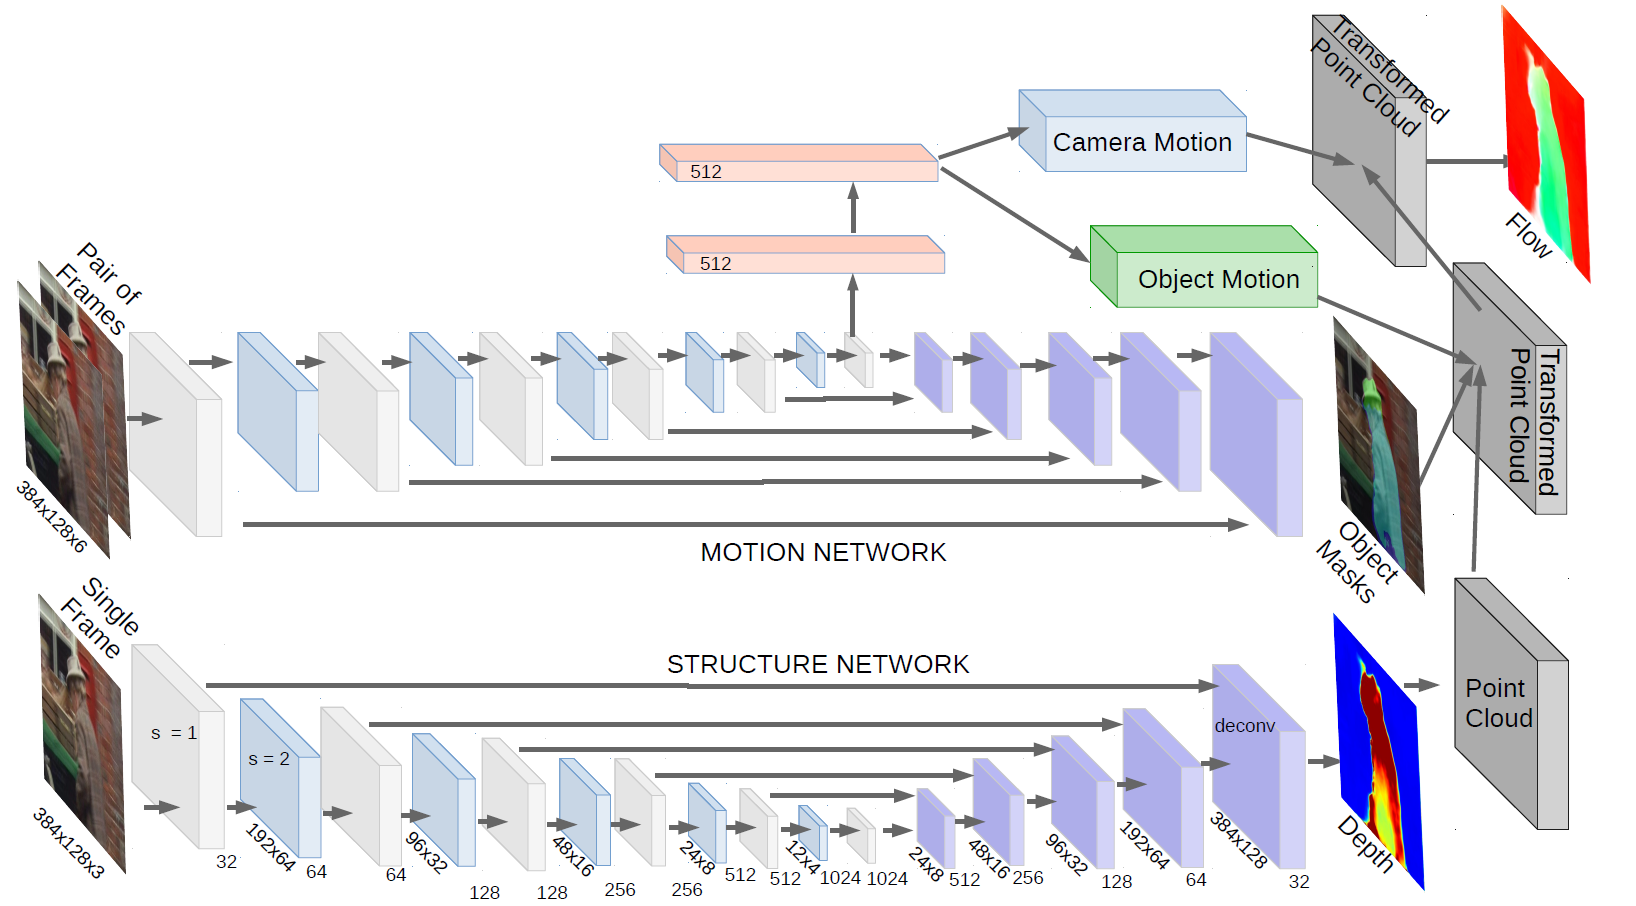
\includegraphics[width=0.9\textwidth]{figs/1-2/sfm-net2.png} 
	\label{sfm-net2}
	\caption{SfM-Net的网络结构图}
\end{figure}

与SfM-Net类似,Yin等人提出的GeoNet~\cite{geonet}自监督学习的方式,利用三维几何约束,将单目深度估计、光流估计和相机运动估计联合学习求解。为了能够恢复出完整场景的光流信息,GeoNet同样将场景显式地分为静态和动态部分,将各种估计通过视角合成生成新视角下的图片,并将损失函数建立在生成图片和拍摄图片的误差上,进行联合的自监督训练。如图~\ref{geonet},GeoNet利用前向和反向两个操作,判断区域内运动是由静态背景还是动态物体造成的,然后分别求解静态和动态部分的光流,合成整个场景的完整光流。另外,为增加对局外点(outlier)、光照变化、遮挡、无纹理和重复纹理区域的鲁棒性,GeoNet还使用了自适应的几何一致性损失函数。目前,GeoNet在室外车辆驾驶环境下,在深度、光流估计上均取得了非常不错的效果。

\begin{figure}[htbp]
	\centering
	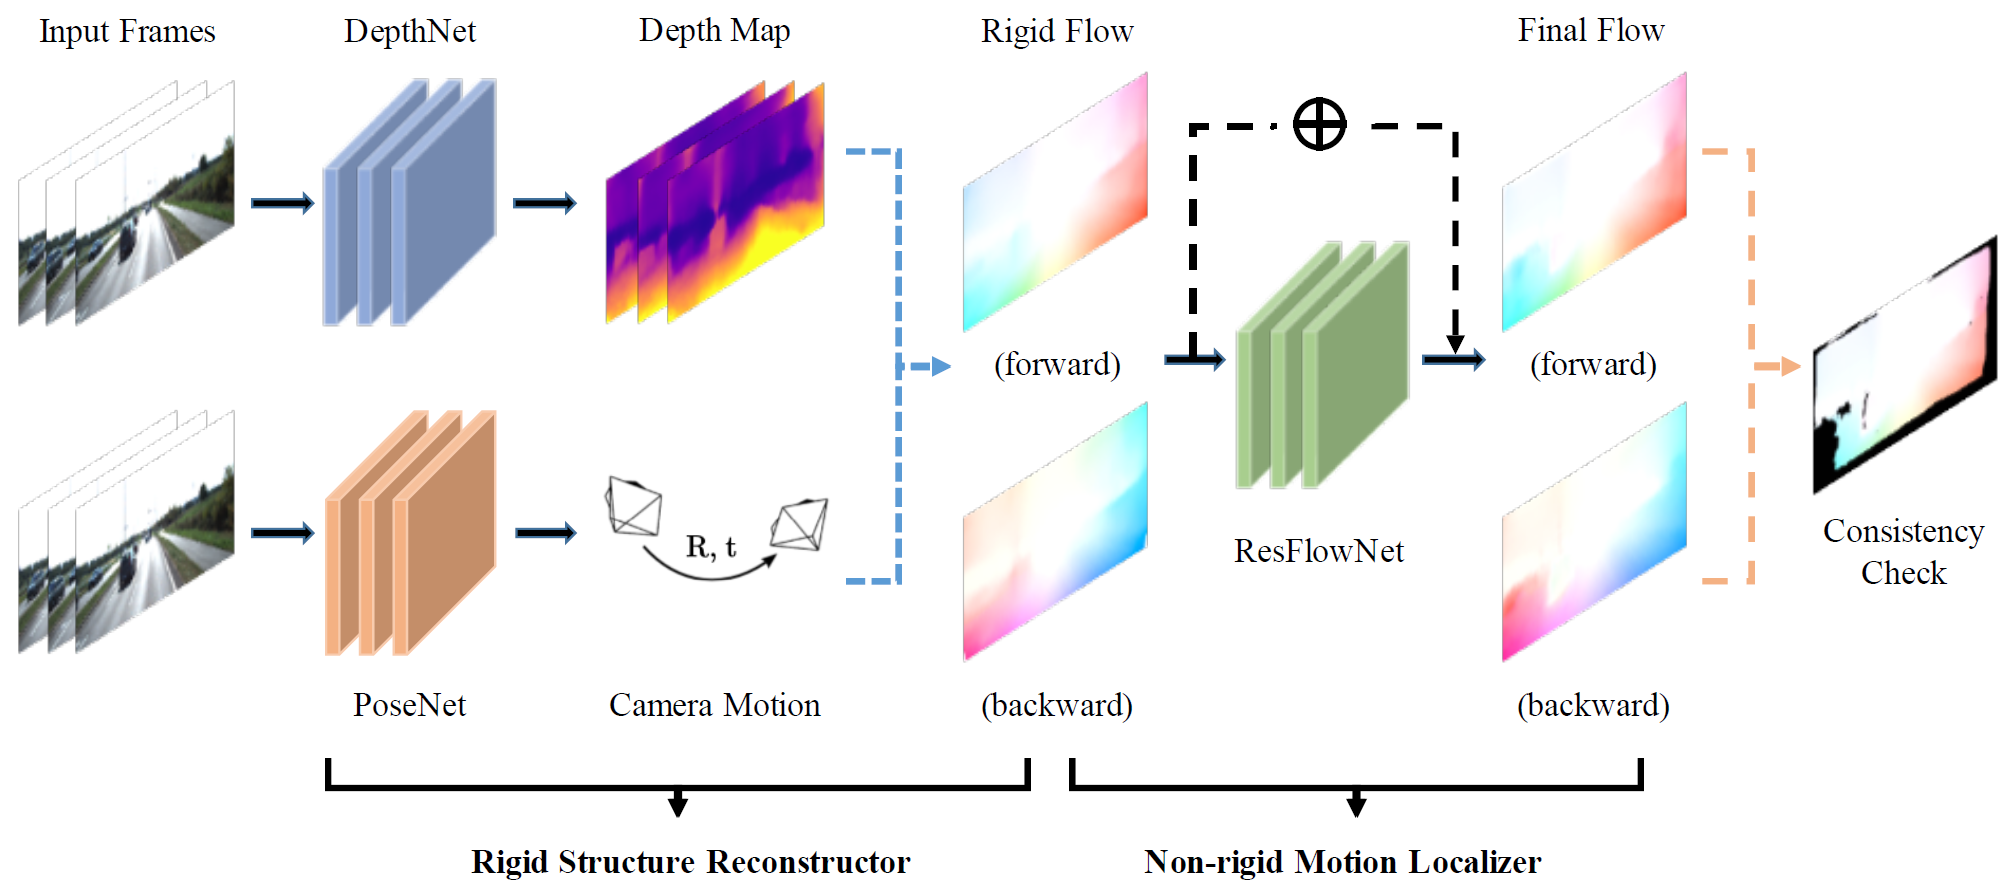
\includegraphics[width=0.9\textwidth]{figs/1-2/geonet.png} 
	\label{geonet}
	\caption{GeoNet的流程图}
\end{figure}

Lai等人认为,双目的深度估计和光流估计有其相同的地方,即寻找对应点的匹配和计算移动距离(视差),而此前的许多工作将二者分别用不同的网络估计,只在损失函数中将其耦合。因此,Lai等人将场景深度估计和光流估计用同一个网络求解~\cite{bridging},共享高维的特征表示,并在SfM-Net和GeoNet这类工作的思路下,充分利用了两个时刻双目图像之间的各种几何约束(如图~\ref{bridge}所示),使光流、深度估计的精度更高,从而有助于动态物体的分割。

\begin{figure}[htbp]
	\centering
	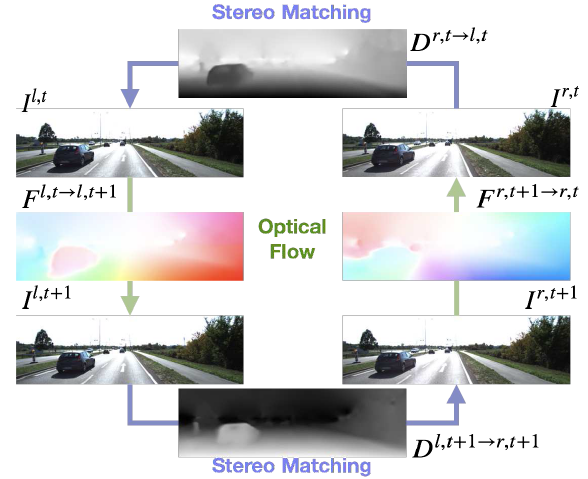
\includegraphics[width=0.43\textwidth]{figs/1-2/bridge1.png}
	\hspace{30pt}
	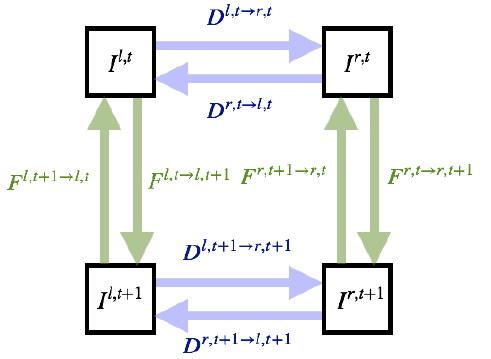
\includegraphics[width=0.43\textwidth]{figs/1-2/bridge2.png}
	\label{bridge}
	\caption{左边为~\cite{bridging}的流程图,右边为该方法利用的各种帧间几何约束}
\end{figure}

最近,Wang等人提出了UnOS网络,同样用双目自监督学习方法联合估计光流和场景深度~\cite{unos}。UnOS使用3个网络同时求解深度、相机位姿和刚性场景下的光流(rigid optical flow),并将刚性光流与FlowNet估计的光流作比较,找出符合刚性场景假设(rigid-scene assumption)即静态的部分。然后,促使两个光流估计在静态部分尽可能一致,那么余下的部分即是动态物体,由此得到动态物体的初步掩膜。之后,使用视觉里程计优化初步估计的掩膜,得到更精准的动态物体分割。在整个自监督训练过程中,除了图片合成作为损失函数之外,UnOS还使用了光流-深度一致性损失函数,使该方法在双目光流、深度估计、动态物体分割任务上均取得了很好的效果。

\begin{figure}[htbp]
	\centering
	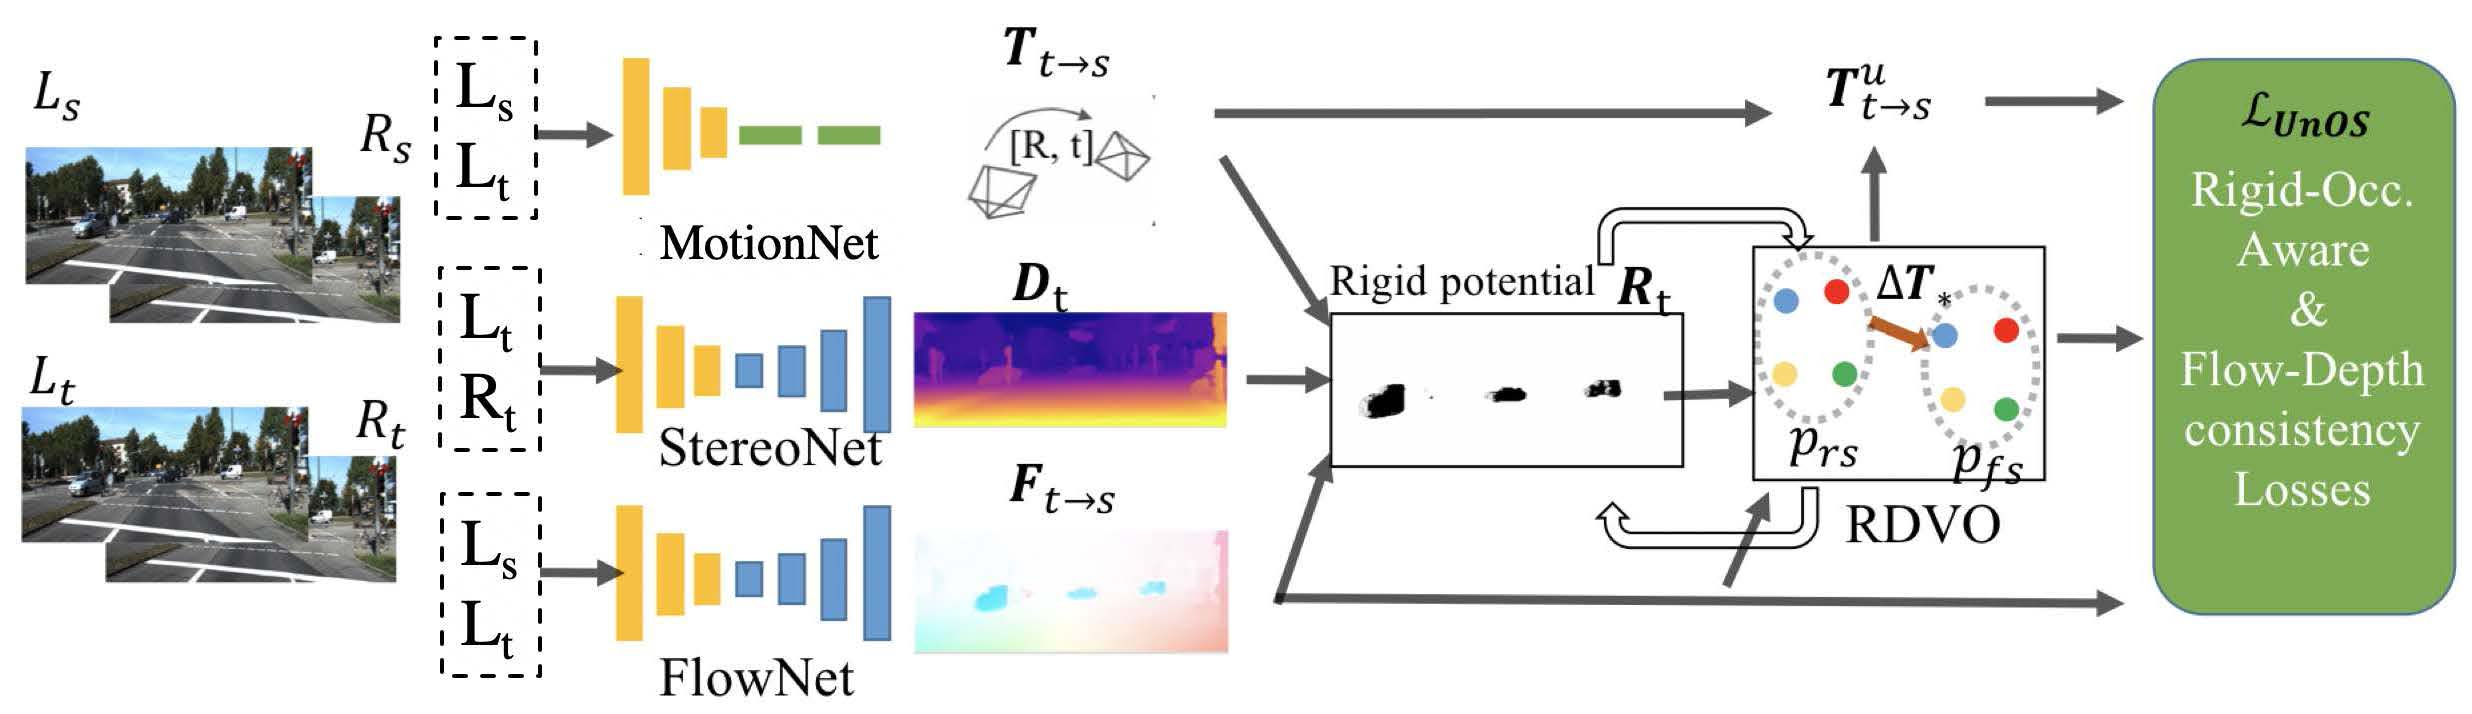
\includegraphics[width=0.9\textwidth]{figs/1-2/unos.jpg} 
	\label{geonet}
	\caption{UnOS的流程图}
\end{figure}



\section{非刚体和多刚体运动下的SfM技术}
\label{subsec:non-rigid_SfM}
为了处理场景中的动态物体,如之前所述将场景中不同运动物体进行分割,并对这些不同运动的物体分别进行三维重建是一个比较直接的方案。但考虑到所有物体的运动和三维信息同时都反应到了视频序列中,理论上这些物体的运动和三维信息可以同时进行求解\cite{Tomasi1992Shape}。在给定特征对应或者像素对应关系的基础上,基于矩阵分解的方式可以从表示了图像序列的特征矩阵中同时求解出动态物体的分割、恢复出各自物体的运动信息以及场景和物体的三维信息。这些方法根据场景三维结构在相机运动的模型下生成图像序列的过程,推导出最终的特征矩阵的特性。根据不同物体运动不同在矩阵中反应出的不同性质,对矩阵进行重新组织,并可以根据图像序列的生成模型将每部分的矩阵分解乘包含了相机运动的矩阵乘以三维信息的形式,利用矩阵中提供的约束同时完成运动物体分割、运动求解以及三维信息恢复。

\subsection{视频序列帧中特征变化的子空间约束}\label{subsec:subspace}
与一般对特征的处理相同,假如我们可以跟踪到视频序列中的一系列特征,比如使用光流等方法\cite{Fanani2016Keypoint},如图\ref{fig:feature_trajectory}所示。为了便于推导,我们在这里假设这些特征在1至f帧之间均连续观测到,噪声和缺失的情况会另外探讨。我们将观测到的特征点记做$x_{ij}=(u_{ij},v_{ij})$,其中下标中$i$代表第$i$帧,$j$代表第$j$个特征点。由于这些特征点是由相机在三维空间中运动生成的,所以这一系列特征点应当连续变化并与三维场景和相机运动对应。我们将这些特征点的坐标根据编号和时间序列排布到一个矩阵中,如式\eqref{eq:measurementMatrix}所示,纵坐标方向上按照帧的时间顺序排列,横坐标按照特征点的编号排列。

\begin{equation}\label{eq:measurementMatrix}
W=
\begin{pmatrix}
u_{11}& \cdots & u_{1p}\\
\vdots& \vdots &\vdots\\
u_{f1}& \cdots & u_{fp}\\
v_{11}& \cdots & v_{1p}\\
\vdots& \vdots &\vdots\\
v_{f1}& \cdots & v_{fp}
\end{pmatrix}
\end{equation}
矩阵分解方法认为这个矩阵是由相机的运动和三维结果矩阵合成而成,可以通过矩阵分解恢复出原始的信息。

\begin{figure}[htbp]
	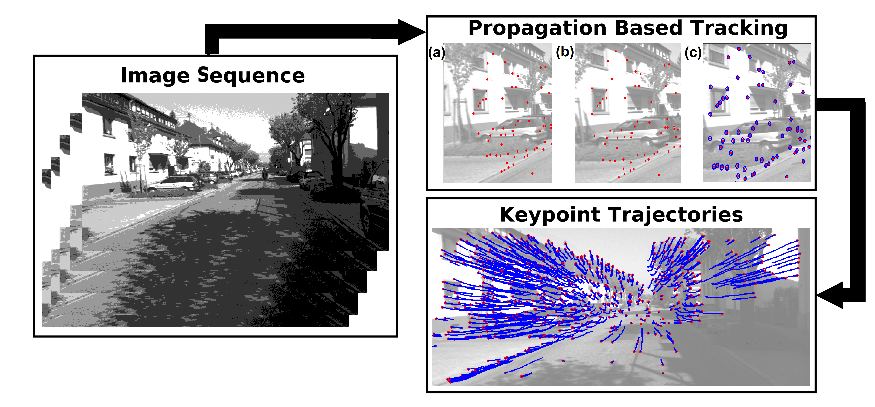
\includegraphics[width=1\textwidth]{figs/1-3/feature_trajectory.png} 
	\caption{跟踪得到的特征点序列轨迹\cite{Fanani2016Keypoint},观测矩阵是将图中连续出现的特征点坐标放到矩阵中,能够表示特征点在空间和时域上的关系。}
	\label{fig:feature_trajectory}
\end{figure}

通过矩阵分解的方式联合求解摄像机运动和三维信息,是SfM中一个重要的方法。这种方法具有优雅的数学描述,充分的考虑到了特征之间在空间和时间上的关联约束。这种方法最早由Tomasi和Kanade\cite{Tomasi1992Shape}根据秩理论在1992年提出。他们的理论指出,在一个面向静态场景的较短的序列中,包含了在整个帧序列上所有跟踪到的特征点的观测矩阵(measurement matrix),它的秩最多是4。特别的对欧式坐标系下的垂直投影来说秩最多是3\cite{Costeira1995A,Tomasi1992Shape,Irani2002Multi,Liu2011Subspace}。这种秩下的约束表明了这些特征点在时间变化是有明显关联的。
\subsection{观测矩阵与相机运动及三维结构的关系}\label{subsec:measurementMatrix}
观测矩阵是由相机的运动和三维点共通生成的,本节主要讲观测矩阵与这两个信息之间有什么样的关系。
由于垂直投影垂直投影形式较为简单,故我们先从垂直投影的情形来做说明\cite{Tomasi1992Shape}。垂直投影的形式如式\eqref{eq:orthogonalProjection}所示,是三维点的$x,y$分量的直接映射。
\begin{equation}\label{eq:orthogonalProjection}
x_j=
\begin{pmatrix}
R_{11} & R_{12} & R_{13} & t_1\\
R_{21} & R_{22} & R_{23} & t_2
\end{pmatrix}
\begin{pmatrix}
X_j\\Y_j\\Z_j\\1
\end{pmatrix}
\end{equation}
其中$R_{ij}$是旋转矩阵$R$的第$(i,j)$个元素,$t_i$是平移分量的元素,上述矩阵中仅包含了旋转矩阵的前两行,第三行可以用这两行的叉乘求得。$[X_j,Y_j,Z_j,1]$是第j个三维点齐次坐标,我们把第j个三维点的齐次坐标写作$X_j$,则对第n帧中的p个点来说,三维点的齐次坐标集合可以写作$[X_1,\cdots,X_p]\in \mathbb{R}^{4\times p}$。设$R_x^j$和$R_y^j$分别代表了第j帧姿态的旋转矩阵的第一行和第二行,$t_x^j$和$t_y^j$代表了第j帧姿态的平移分量。我们对每个相机对整个三维点集用式\eqref{eq:orthogonalProjection}进行投影,将得到的二维点堆叠起来就可以得到式\eqref{eq:measurementMatrix}中的观测矩阵,如式\eqref{eq:orthogonalMeasurementMatrix}所示。

\begin{equation}\label{eq:orthogonalMeasurementMatrix}
\begin{pmatrix}
u_{11}& \cdots & u_{1p}\\
\vdots& \vdots &\vdots\\
u_{f1}& \cdots & u_{fp}\\
v_{11}& \cdots & v_{1p}\\
\vdots& \vdots &\vdots\\
v_{f1}& \cdots & v_{fp}
\end{pmatrix}
=
\begin{pmatrix}
{R_x^1}^T & t_x^1\\
\vdots & \vdots\\
{R_x^f}^T & t_x^f\\
{R_y^1}^T & t_y^1\\
\vdots & \vdots\\
{R_y^f}^T & t_y^f\\
\end{pmatrix}
\begin{pmatrix}
X_1&\cdots &X_p
\end{pmatrix}
\end{equation}


一个更复杂的情况是在仿射相机(affine camera)的模型下进行推导\cite{Feng2013Joint}。在这个假设下,相机的投影模型可以简化成如式\eqref{eq:affineCameraModelProjection}所示的形式,旋转矩阵中最后一行为0。
\begin{equation}\label{eq:affineCameraModelProjection}
x_j=\pi
(
\begin{pmatrix}
f & 0 & c_1\\
0 & f& c_2\\
0 & 0 &1
\end{pmatrix}
\begin{pmatrix}
R_{11} & R_{12} & R_{13} & t_1\\
R_{21} & R_{22} & R_{23} & t_2\\
0      & 0      & 0      & d_0
\end{pmatrix}
\begin{pmatrix}
X_j\\Y_j\\Z_j\\1
\end{pmatrix}
)
\end{equation}
其中$f$是相机的焦距,$(c_1,c_2)$是图像中心,$d_0\in \mathbb{R}$ 是一个常量,$R_{ij}$是旋转矩阵$R$的第$(i,j)$个元素,$t_i$是平移分量的元素,$\pi(\cdot)$是讲齐次量变化为非齐次量的过程,即$\pi([X,Y,Z]=[X/Z,Y/Z])$。
我们定义如下的观测矩阵,其中每个位置为当前帧的二维位置减去第一帧的位置$x_{ij}-x_{1j}$。则对每一个三维点$X_j$来说这组观测矩阵元素可以写成式\eqref{eq:affineMearuement}。
\begin{eqnarray}\label{eq:affineMearuement}
\begin{pmatrix}
u_{ij}\\
v_{ij}
\end{pmatrix}
&=&
x_{ij}-x_{1j}\\
&=&\frac{f}{d_0}
\begin{pmatrix}
(R_{11}^i-1)X_{j}+R_{12}^i Y +R_{13}^i Z_j+t_x^i\\
R_{21}X_j + (R_{22}^i-1)Y_j+R_{23}^i Z_j+t_x^i
\end{pmatrix}
\end{eqnarray}
则显然的在仿射投影关系下,观测矩阵也是由包含姿态的矩阵乘以包含了三维点信息的矩阵得到。

对投影相机来说,上述的简单关系更复杂一些,因为齐次化过程依赖于每个像素的深度信息\cite{Sturm1996A}。考虑到齐次坐标到非齐次坐标的变换,为了能够通过矩阵分解的方式进行求解,我们把齐次化中的尺度因子作为一个需要先求解的参数进行处理。我们把投影关系下的尺度因子记做$\lambda\in \mathbb{R}$。我们记${P_i\in \mathbb{R}^{3\times4}}_{i=1}^f$ 是一系列相机的投影矩阵,包含了旋转和投影及内参的关系,把齐次坐标表示的三维点${X_j\in \mathbb{R}^4}_{j=1}^p$映射到第i个相机里,即满足投影关系$\lambda_{ij}x_{ij}=P_i X_j$。在整个视频序列以及整个三维点集上完整的投影投影过程如式\eqref{eq:projectiveMeasurementMatrix}所示,
\begin{equation}\label{eq:projectiveMeasurementMatrix}
W=
\begin{pmatrix}
\lambda_{11}x_{11}&\cdots&\lambda_{1p}x_{1p}\\
\vdots&\ddots & \vdots\\
\lambda_{f1}x_{f1}&\cdots&\lambda_{fp}x_{fp}
\end{pmatrix}
=
\begin{pmatrix}
P_1\\
\vdots\\
P_f
\end{pmatrix}
\begin{pmatrix}
X_1,&\cdots,&X_p
\end{pmatrix}.
\end{equation}

Sturm 和 Trigss\cite{Sturm1996A} 根据基本矩阵和极点的约束对式\eqref{eq:projectiveMeasurementMatrix}中的$\lambda$进行了求解。由于单目视频本来就无法恢复尺度,我们可以任意选择一个深度尺度,比如设$\lambda_{1p}=1$作为初始值。根据不同帧之间的极线约束,这些射影相机观测矩阵中的深度尺度可以按照式\eqref{eq:projectiveDepthUpdate}进行更新求解:
\begin{equation}\label{eq:projectiveDepthUpdate}
\lambda_{mp}=\frac{(e_{mn}\times x_{mp})\cdot(F_{mn}x_{np})}{\Vert e_{mn}\times x_{mp}\Vert}\lambda_{np}.
\end{equation} 
其中$m,n\in{1,2,\cdots,f}$,$F_{mn}$和$e_{mn}$分别为$m$对$n$帧之间定义的基本矩阵和极点。在求解得所有的深度尺度$\lambda_{mp}$之后我们就可以得到射影相机模型下的观测矩阵。

针对射影相机的另一个处理方式是Liu等人\cite{Feng2013Joint}所采用的小运动近似的方式。这种方式中假设在视频序列中相机的运动相对与帧率来说非常缓慢,每帧之间的旋转运动较小,可以使用李代数到旋转矩阵的一阶泰勒展开做为近似,在这个近似下线性关系更加明确,能够得到简单的观测矩阵。
\subsection{针对多刚体系统的观测矩阵分解}
我们先从静态世界或者整体就是一个刚体的系统进行考虑,通过\ref{subsec:subspace}节的方式,我们可以在一个视频序列中得到它的观测矩阵$W\in \mathbb{R^{2f\times p}}$,这里$f$是帧数$p$是三维点数。根据\ref{subsec:measurementMatrix}节中的推导,我们可以看出这个观测矩阵可以分解成运动矩阵$M\in \mathbb{R}^{2f\times 4}$和形状矩阵$S\in\mathbb{R}^{4\times p}$即如式\eqref{eq:Factorization}所示:
\begin{equation}\label{eq:Factorization}
W=M S .
\end{equation}

在求解过程中,我们在得到观测矩阵$W$之后,基于秩约束(Rank constraint)\cite{Costeira1998A},矩阵$W$可以用奇异值分解(SVD)进行分解,得到
\begin{equation}\label{eq:svdFactorization}
W=U\Sigma V,
\end{equation}
的形式。其中$\Sigma\in \mathbb{R}^{4\times4}$是一个对角阵,包含了最大的四个特征值,$U\in \mathbb{R}^{2f\times4}$和$V\in \mathbb{R}^{p\times4}$是对应到最大的四个特征值的特征向量。之后我们可以用$\hat{M}=U\Sigma^{1/2}$和$\hat{S}=\Sigma^{1/2}V^T$来表示运动矩阵和形状矩阵。但是式\eqref{eq:svdFactorization}中的分解并不是唯一的,真实的运动矩阵$M$和形状矩阵$S$还需要再找到一个映射矩阵$A$使得整个分解过程如下式所示:
\begin{equation}
W=M S=(\hat{M}A)(A^{-1}\hat{S}).
\end{equation}
其中矩阵$A$可以通过旋转矩阵和平移所带有的先验约束进行求解,并可以转化成一个最小二乘形式线性求解过程\cite{Costeira1998A,Tomasi1992Shape}。

上述就是通过分解形式联合求解静态场景问题的基本框架,这个框架可以比较容易的推广到场景中存在独立运动的多个刚体的情形\cite{Costeira1998A}。我们假设场景中包含了$n$个独立运动的刚体,则我们可以通过列交换的形式把观测矩阵$W$中的特征序列根据刚体分组成$[W_1,\cdots,W_n]$,这个过程可以用一个排列矩阵$\Gamma$来表示,如式\eqref{eq:multibodyMeasurementMatrix}所示,其中$\Gamma\in \mathbb{R}^{p\times p}$是一个未知的排列矩阵。
\begin{equation}\label{eq:multibodyMeasurementMatrix}
\bar{W}=W \Gamma=\begin{pmatrix}
W_1,\cdots,W_n
\end{pmatrix}
\end{equation}

在没有噪声的情况下,每一个独立的$W_i$即和前述静态场景中的观测矩阵等价应当在一个秩不超过4的子空间中。这样每个$W_i$可以进行单独的分解,得到该刚体的运动矩阵$M_i$以及形状矩阵$S_i$,如下式所示:
\begin{equation}\label{eq:multibodyFactorization}
\bar{W}=\bar{M} \bar{S} = 
\begin{pmatrix}
M_1,\cdots,M_n
\end{pmatrix}
\begin{pmatrix}
	S_1 & &\\
	&\ddots&\\
	&      &S_n
\end{pmatrix}
.\end{equation}
这样对多刚体运动的问题来说,最关键的就是求解排列矩阵$\Gamma$让分解得到的矩阵$\bar{S}$具有块对角的性质。

多刚体运动恢复结构(Multibody Structure from Motion)对标准SfM下刚体相机的运动进行了拓展,变成了n个刚体的刚性运动模型。为了解决多刚体运动恢复结构问题,在仿射相机模型的假设下Costeira和Kanade\cite{Costeira1998A} 引入了一个形状交互矩阵的概念。这个理论里对物体形状构造了一个数学上的可证明的、对刚体运动具有不变性、不依赖于坐标系的描述。这里的结构交互矩阵被证明可以保持在原始子空间里的结构。我们设$\bar{W}=U\Sigma V^T$是一个秩r的观测矩阵SVD分解结果,其中$U\in \mathbb{R}^{2f\times r}$, $\Sigma\in \mathbb{R}^{r\times r}$,$V\in \mathbb{R}^{p\times r}$。则形状交互矩阵$Q$就可以定义为:
\begin{equation}\label{eq:shapeInteractionMatrix}
Q=VV^T\in \mathbb{R}^{p\times p}.
\end{equation}
式\eqref{eq:shapeInteractionMatrix}具有一个特殊的形状,当两个特征序列分别属于是两个刚体的时候,$Q$的元素会是0。 这个特性可以在数学上得到证明\cite{Kanatani2001Motion}。 在这个理论基础上,矩阵分解的求解过程可以基于对$Q$的排序和元素大小的限制来或得不同刚体的分割以及三维信息的重建。
在\cite{Costeira1998A}中,这种运动刚体的分割和聚类是通过最大化式\eqref{eq:multibodyFactorization}中$S$的对角元素,并且利用$Q$来约束对角线上的每个块应当属于不同的刚体的约束这样的方式进行求解。Ichimura\cite{Ichimura1999Motion} 使用在\cite{Ostu2007A}中最大化不同子空间的差异性的判别准则将$Q$中的不同刚体到不同的刚体。
\subsection{针对非刚性运动的观测矩阵分解}
假如场景中的物体是非刚性运动的时候,情况会非常复杂。Bregler\cite{Bregler2013Recovering}等针对非刚性运动恢复结构上针对垂直投影相机提出了第一个观测矩阵分解的方式。他们的核心想法是将一个非刚体的物体表示成一组基的组合,认为这个刚体在这些帧中的运动过程可以在这个状态空间中进行近似表示。比如我们选择$k$个关键帧中的结构作为一组基${B_i}_{i=1}^k$,其中每个$B_i$代表了一个$3\times p$的矩阵,表示了$p$个特征点。这组基的线性组合$B=\sum_{i=1}^k{l_i B_i}$可以确定一个刚体的描述,其中$l_i\in \mathbb{R}$是一组系数。通过\cite{Tomasi1992Shape}中的方法进行中心化并消去平移向量之后,可以将观测矩阵表示成式\eqref{eq:nonrigidMeasurementMatrix}所示:
\begin{equation}\label{eq:nonrigidMeasurementMatrix}
\tilde{W}=N B=
\begin{pmatrix}
l_{11}R'_1 &\cdots & l_{1k}R_1'\\
\vdots & \ddots & \vdots\\
l_{f1}R'_f & \cdots &l_{fk}R'_f
\end{pmatrix}
\begin{pmatrix}
B_1\\
\vdots\\
B_k
\end{pmatrix}.
\end{equation}
其中$R'$是旋转矩阵的前两行,由于垂直投影的假设这里R就是旋转矩阵不包含内参的过程,所以旋转矩阵的第三行可以通过前两行的叉乘得到。针对观测矩阵$\tilde{W}$进行SVD分解,根据秩3的约束,我们选择3个最大的奇异值及对应的特征向量。则旋转矩阵元素$R_i'$和形状基的系数$l_ij$可以从$N$中,通过重新排列$N$的顺序并且对它进行SVD分解恢复出来。与刚性问题中面临同样的问题即SVD可以得到的结果是不唯一的,最后可以通过正交约束求解得到一个映射矩阵$G$得到$R_f'$和$B_k$的唯一解。另一中约束是\cite{Xiao2006A}中引入了一个新的基约束,使得非刚性的分解问题能够使用闭解的形式进行求解。除了直接使用度量约束(metric constraints),Paladini等\cite{Paladini2009Factorization}将运动矩阵投影到一个矩阵流形的约束上,让整个分解过程可以通过迭代的方式进行处理。在这些工作的基础上,Dai等\cite{Dai2012A}尝试去掉针对非刚性重建的额外假设,比如之前使用的非刚性基、针对非刚性场景的先验等,提出了一个没有额外先验的仅使用低秩约束的方法。Kumar等\cite{Kumar2016Multi}提出了融合多刚体和非刚体的方法,将问题建模成多个非刚体变换的系统。他们讲整个特征轨迹建模乘联合的多个线性或者仿射的空间。可以允许同时优化非刚性的重建和刚性的重建。


\chapter{长时变化环境下的地图更新}
\label{sec:mapping}
\subsection{动态环境下静态部分地图的构建}
\label{subsec:object-centered_mapping}
\subsection{静态背景和动态物体的同时重建}
\label{subsec:static_and_dynamic}
\section{四维地图构建与长时定位}
\label{subsec:4Dmapping}


\bibliographystyle{unsrt}
\bibliography{mybibfile}
	
\end{document}